
\section{Sanity Check}
We first wanted to ensure that the changes made to the neural network architecture to incorporate reward decomposition resulted in learning comparable to that of an agent trained without decomposed rewards. To this end, in the Highway environment, we compared the cumulative rewards of two RL agents that differ only by their neural network architecture. To correctly compare the single-value reward to the decomposed reward, we normalized the decomposed rewards so that the sum of all available reward components approximately equals the available single-value reward. Table ~\ref{tab:valus_Original_vs_Multi} presents the main parameters that were used for each RL agent.
The results show that the average reward of an RL agent with multiple heads is in the same range as an RL agent that uses a traditional neural network (see Table~\ref{tab:valus_Original_vs_Multi}).
We can conclude from this check that in our domain using reward decomposition did not harm the performance of the agent.



\section {Satisfaction Results}


The results of the Explanation Satisfaction scale are shown in Figure \ref{fig:satisfaction}. 

\begin{figure}[h]
\begin{minipage}{0.49\linewidth}
\centering

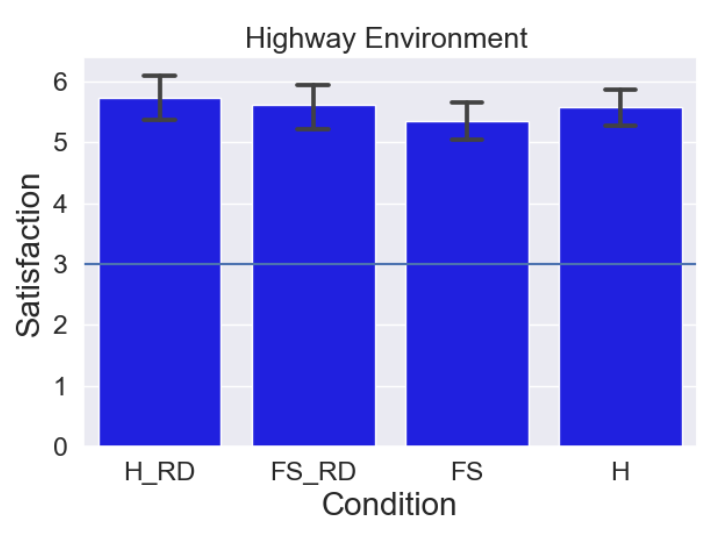
\includegraphics[width=\linewidth]{Highway_env_satisfaction.PNG}

(A)

\end{minipage}
\begin{minipage}{0.49\linewidth}
\centering

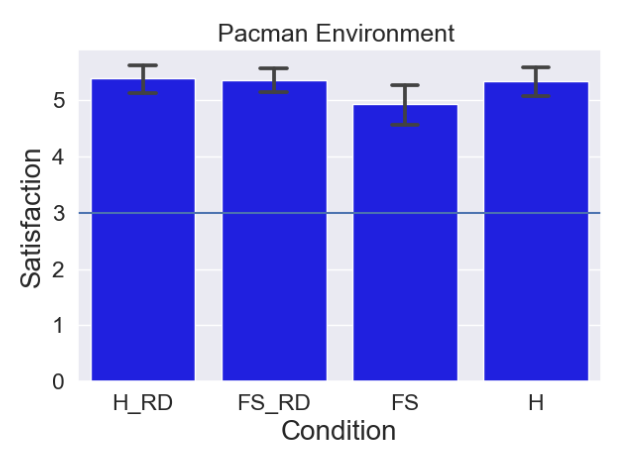
\includegraphics[width=\linewidth]{Pacman_env_satisfaction.PNG}

(B)
\end{minipage}
\caption{Participants' explanation of satisfaction by conditions in the Highway environment (A) and in the Pacman environment (B). The error bars show the 95\% CI. }
\label{fig:satisfaction}
    \vspace{-0.2cm}
\end{figure}

\section{Survey Information}
\label{ap:survey_information}
The following figures are screenshots from the Pacman environment survey under the condition of Highlight explanation.
As an example, we show the survey only for the Highlight condition and only included one of the agents.
The participants were shown multiple different agents and depending on their condition they saw explanations as shown in Figure \ref{fig:Survey_example_Pacman}.
The Highway environment survey was conducted similarly to the survey that is presented here.

\begin{figure}[]
\centering
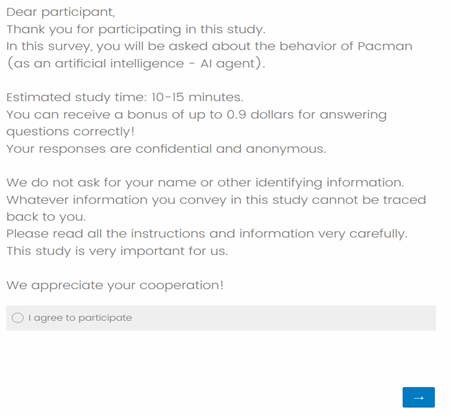
\includegraphics[width=0.7\linewidth]{consent.png}
\end{figure}
\begin{figure}[t]
\centering
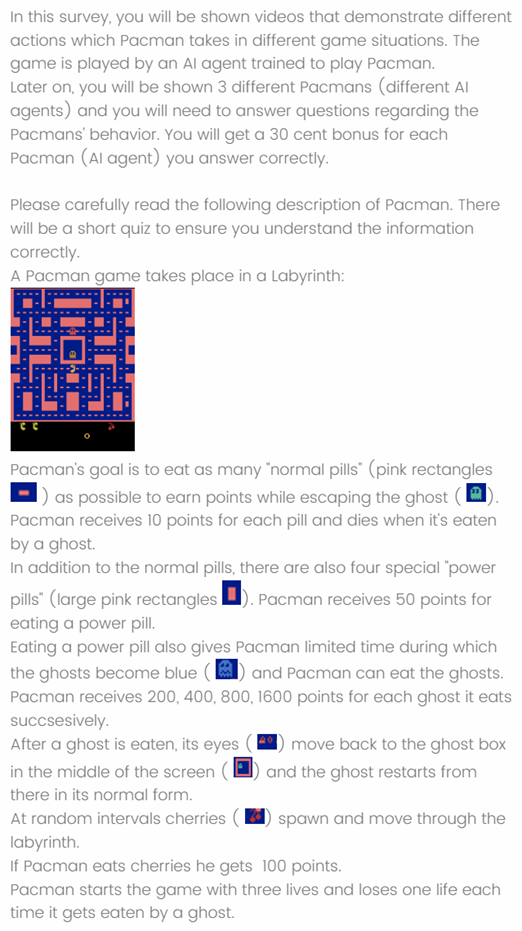
\includegraphics[width=0.7\linewidth]{pacman_domain.png}
\end{figure}
\begin{figure}[t]
\centering
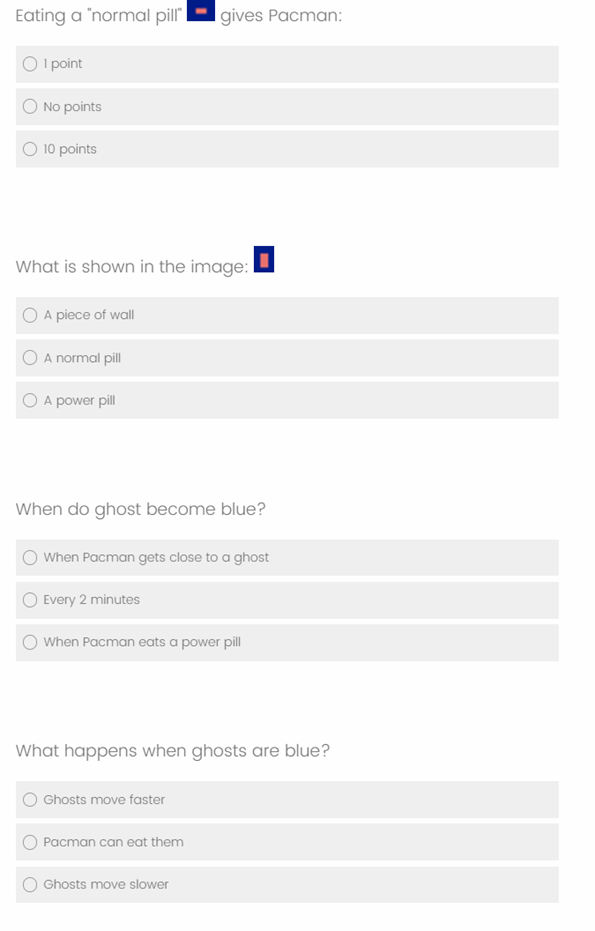
\includegraphics[width=0.7\linewidth]{domain_q.png}
\end{figure}
\begin{figure}[t]
\centering
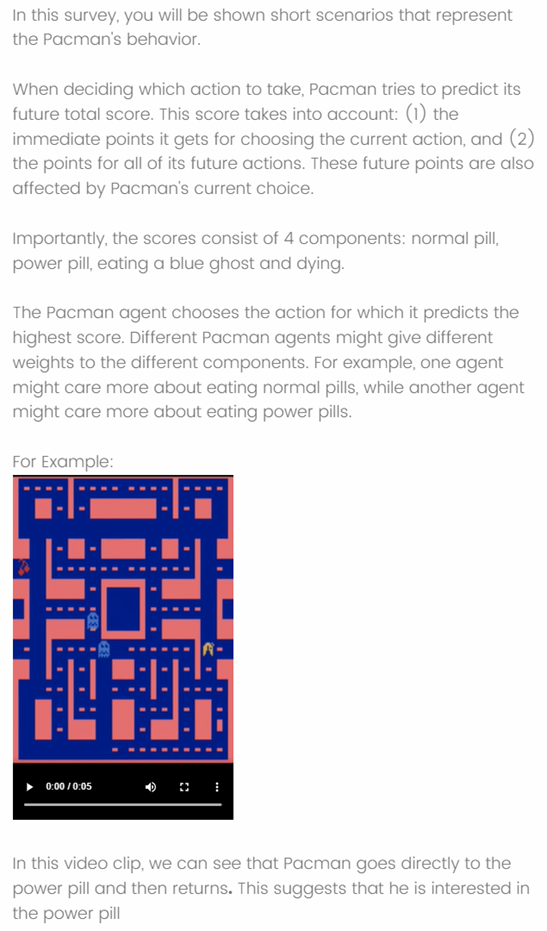
\includegraphics[width=0.7\linewidth]{survey.png}
\end{figure}
\begin{figure}[t]
\centering
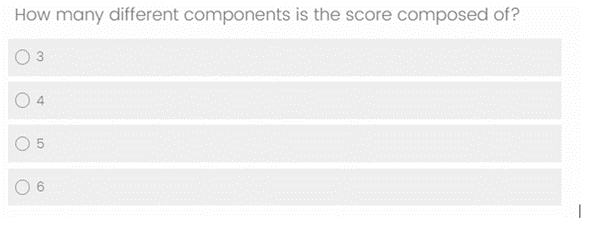
\includegraphics[width=0.7\linewidth]{survey_q.png}
\end{figure}
\begin{figure}[t]
\centering
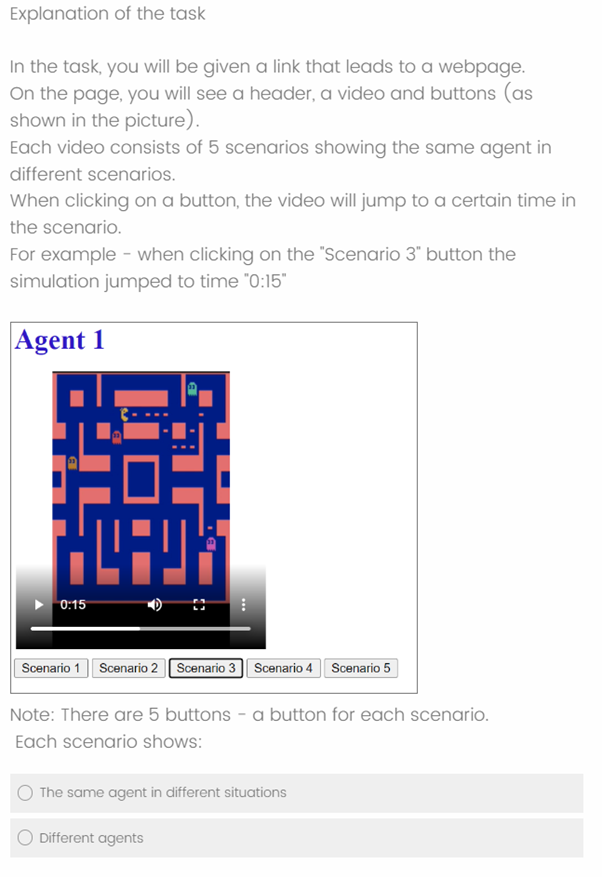
\includegraphics[width=0.7\linewidth]{expla_task.png}
\end{figure}
\begin{figure}[t]
\centering
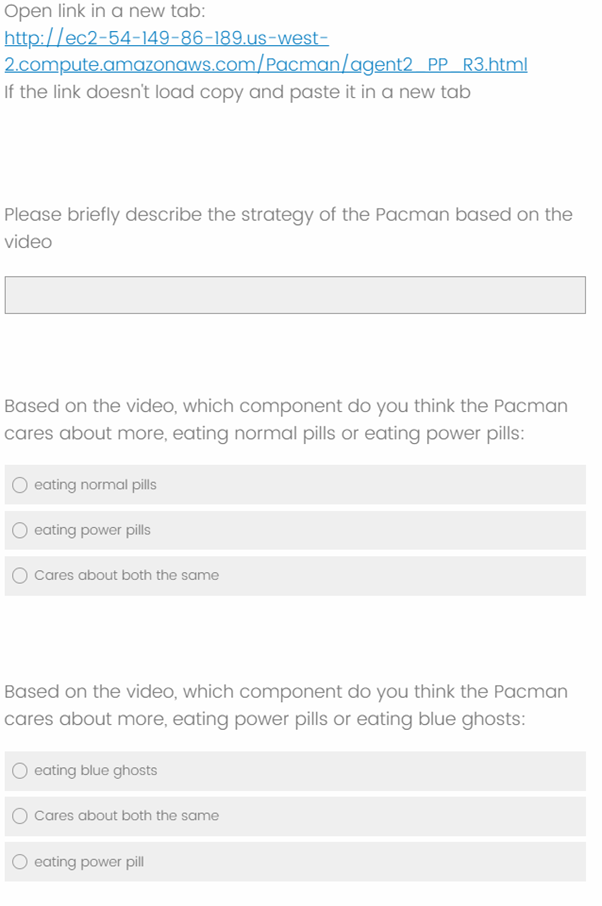
\includegraphics[width=0.7\linewidth]{agent_q_1.png}
\end{figure}
\begin{figure}[t]
\centering
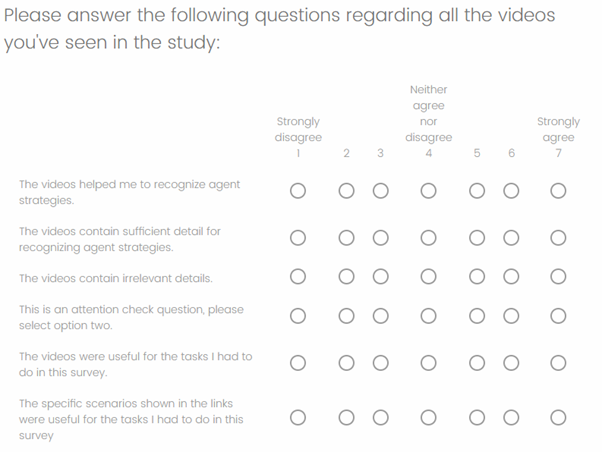
\includegraphics[width=0.7\linewidth]{sat_q.png}
\end{figure}

\clearpage

\begin{table*}[!ht]
\centering
\begin{tabular}{c|c c }
%\begin{tabular}{p{5cm}|p{5cm} p{5cm} }
\hline

 & Original & Multiple Heads \\
\hline
Type & Multi Layer Perceptron & Multi Layer Perceptron\\

Method & Epsilon Greedy & Epsilon Greedy\\

Loss function & L2 & L2\\

Duration of each episode&40 time stamps&40 time stamps\\

Number of lanes & 4 & 4\\

Number of vehicles & 30 & 30\\
\hline
& & head 1 right lane=5\\
& right lane=5&  head 1 high speed=0\\
& &head 1 lane change=0\\ \cline{2-3}
& & head 2 right lane=0\\
Reward& high speed=5&  head 2 high speed=5\\
& & head 2 lane change=0\\ \cline{2-3}
& & head 3 right lane=0\\
& lane change=5 &  head 3 high speed=0\\
& &head 3 lane change=5\\ 
\hline
Reward normalization range &[0,1]&[0,1/3]-for each reward component\\

Number of episodes&2000&2000\\

Average result of reward & 38 & 39\\

\hline
\end{tabular}
\caption{Main values and results of RL agent with original neural network vs. multi-head neural network}
\label{tab:valus_Original_vs_Multi}
\end{table*}

\section{Highway Environment}
\label{ap:highway_env}

In the Highway environment, we used the following parameters:
\begin{itemize}
\item Number of lanes = 4
\item Vehicles count = 30
\item Duration = 40
\item Ego spacing = 2
\item Vehicles density =1
\item Simulation frequency= 15
\item Policy frequency=15
\end{itemize}
